% Diagram for the report (pipeline). Build: see build.sh in this folder.
\documentclass[12pt]{standalone}
% Shared style of every diagram and chart in the report.
% Each agent keeps the same colour in every figure.
% The diagrams are drawn here, not in main.tex, so the report itself does not
% load TikZ: it includes the built PDFs and compiles within Overleaf's time limit.
\usepackage{amsmath,amssymb}
\usepackage{xcolor}
\usepackage{tikz}
\usetikzlibrary{positioning,arrows.meta,shapes.geometric,shapes.misc,fit,calc,backgrounds}
\usepackage{pgfplots}
\pgfplotsset{compat=1.18}

% Same text width as the report (A4, 30 mm + 20 mm margins), for the charts.
\setlength{\textwidth}{160mm}
\newcommand{\Rs}{Rs.\,}
\newcommand{\code}[1]{\texttt{\detokenize{#1}}}

\definecolor{ink}{HTML}{2B2B2B}
\definecolor{agAfill}{HTML}{E4F2E1}\definecolor{agAline}{HTML}{3E7D3A} % Agent 1 Document & Vendor
\definecolor{agBfill}{HTML}{FCEBD5}\definecolor{agBline}{HTML}{B8701D} % Agent 2 Approval & Inventory
\definecolor{agCfill}{HTML}{EEE4F4}\definecolor{agCline}{HTML}{6E4A8E} % Agent 3 Contract & Risk
\definecolor{agDfill}{HTML}{FBE4E4}\definecolor{agDline}{HTML}{A8474B} % Agent 4 Platform
\definecolor{infill}{HTML}{E8EDF6}\definecolor{inline}{HTML}{4F6188}    % infrastructure / data
\definecolor{exfill}{HTML}{F2F2F2}\definecolor{exline}{HTML}{6F6F6F}    % people and external systems
\definecolor{humfill}{HTML}{FFF6D6}\definecolor{humline}{HTML}{9A7B12}  % human decision points
\definecolor{chartA}{HTML}{9AA5B1}\definecolor{chartB}{HTML}{3F5E8C}    % chart: baseline / shipped

\tikzset{
  >={Stealth[length=2mm]},
  every picture/.style={font=\footnotesize, line width=0.6pt, draw=ink, text=ink},
  nohyph/.style={execute at begin node={\hyphenpenalty=10000\exhyphenpenalty=10000}},
  box/.style={nohyph, draw, rounded corners=2pt, align=center, inner sep=3pt, minimum height=8mm},
  agA/.style={box, fill=agAfill, draw=agAline},
  agB/.style={box, fill=agBfill, draw=agBline},
  agC/.style={box, fill=agCfill, draw=agCline},
  agD/.style={box, fill=agDfill, draw=agDline},
  infra/.style={box, fill=infill, draw=inline},
  ext/.style={box, fill=exfill, draw=exline},
  human/.style={box, fill=humfill, draw=humline},
  decision/.style={nohyph, diamond, aspect=2.2, draw=humline, fill=humfill, align=center, inner sep=1pt},
  flow/.style={->, draw=ink},
  dflow/.style={->, draw=ink, dashed},
  lbl/.style={font=\scriptsize\itshape, fill=white, inner sep=1pt},
  note/.style={font=\scriptsize\itshape, align=center},
}
\pgfplotsset{
  reportbars/.style={
    ybar, width=0.95\textwidth, height=6cm, ymin=0,
    enlarge x limits=0.18, bar width=11pt,
    ymajorgrids, grid style={draw=black!12},
    axis line style={draw=black!60}, tick style={draw=black!60},
    legend style={draw=none, font=\footnotesize, legend columns=-1, at={(0.5,1.03)}, anchor=south},
    tick label style={font=\footnotesize}, label style={font=\footnotesize},
    nodes near coords, every node near coord/.append style={font=\scriptsize},
    /tikz/every even column/.append style={column sep=0.6cm},
    legend image code/.code={\draw[#1, draw=none] (0cm,-0.1cm) rectangle (0.3cm,0.1cm);},
  },
}

\begin{document}
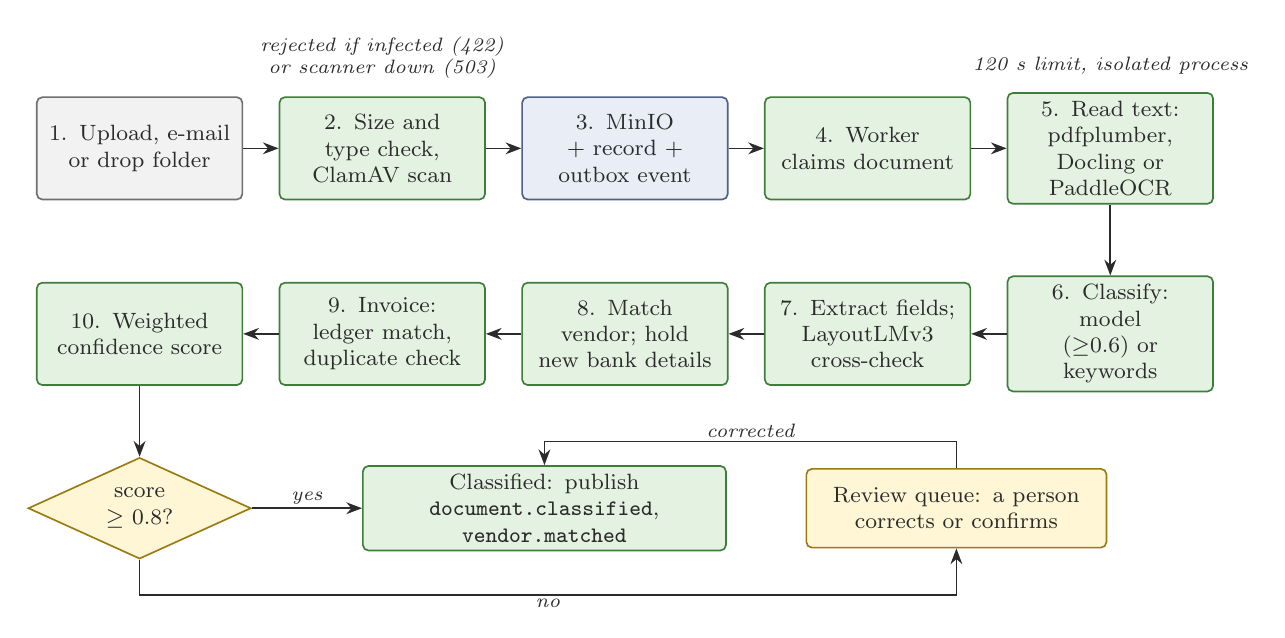
\begin{tikzpicture}[node distance=4.5mm]
\tikzset{st/.style={agA, text width=2.4cm, minimum height=13mm}}
\node[ext, text width=2.4cm, minimum height=13mm] (s1) {1. Upload, e-mail or drop folder};
\node[st, right=of s1] (s2) {2. Size and type check, ClamAV scan};
\node[infra, text width=2.4cm, minimum height=13mm, right=of s2] (s3) {3. MinIO + record + outbox event};
\node[st, right=of s3] (s4) {4. Worker claims document};
\node[st, right=of s4] (s5) {5. Read text: pdfplumber, Docling or PaddleOCR};
\node[st, below=9mm of s5] (s6) {6. Classify: model\\($\geq$0.6) or keywords};
\node[st, left=of s6] (s7) {7. Extract fields; LayoutLMv3 cross-check};
\node[st, left=of s7] (s8) {8. Match vendor; hold new bank details};
\node[st, left=of s8] (s9) {9. Invoice: ledger match, duplicate check};
\node[st, left=of s9] (s10) {10. Weighted confidence score};
\node[decision, below=9mm of s10, text width=1.5cm] (d) {score\\$\geq$ 0.8?};
\node[agA, text width=4.4cm, minimum height=10mm, right=14mm of d] (ok) {Classified: publish \code{document.classified}, \code{vendor.matched}};
\node[human, text width=3.6cm, minimum height=10mm, right=10mm of ok] (rev) {Review queue: a person corrects or confirms};
\foreach \a/\b in {s1/s2,s2/s3,s3/s4,s4/s5,s5/s6,s6/s7,s7/s8,s8/s9,s9/s10,s10/d} \draw[flow] (\a) -- (\b);
\draw[flow] (d) -- node[lbl, above] {yes} (ok);
\draw[flow] (d.south) -- ++(0,-0.45) -| node[lbl, pos=0.25, below] {no} (rev.south);
\draw[flow] (rev.north) |- node[lbl, pos=0.75, above] {corrected} ($(ok.north)+(0,0.3)$) -- (ok.north);
\node[note, above=1mm of s2] {rejected if infected (422)\\or scanner down (503)};
\node[note, above=1mm of s5] {120 s limit, isolated process};
\end{tikzpicture}
\end{document}
